\documentclass{scrreprt}
\usepackage{listings}
\usepackage{underscore}
\usepackage{graphicx}
\usepackage[bookmarks=true]{hyperref}
\usepackage[utf8]{inputenc}
\usepackage[english]{babel}
\usepackage{float}
\hypersetup{
    bookmarks=false,    % show bookmarks bar?
    pdftitle={Beatysys: A system for Cosmetic Surgery Clinics},    % title
    pdfauthor={De La Mora Vazquez Victor Manuel \\ Noyola barradas Juan Diego \\ Ruiz Alvarez Jose Eduardo \\ Toledo Perez Cristian Alejandro \\ Velazquez Gonzalez Jesus Alejandro},                     % author
    pdfsubject={TeX and LaTeX},                        % subject of the document
    pdfkeywords={TeX, LaTeX, graphics, images}, % list of keywords
    colorlinks=true,       % false: boxed links; true: colored links
    linkcolor=blue,       % color of internal links
    citecolor=black,       % color of links to bibliography
    filecolor=black,        % color of file links
    urlcolor=purple,        % color of external links
    linktoc=page            % only page is linked
}%
\def\myversion{1.0}
\date{}
%\title
\usepackage{hyperref}
\begin{document}

\begin{flushright}
    \rule{16cm}{5pt}\vskip1cm
    \begin{bfseries}
        \Huge{BEATYSYS: A system for Cosmetic Surgery Clinics}\\
        \vspace{1.5cm}
        for\\
        \vspace{1.5cm}
        TaskLab\\
        \vspace{1.5cm}
        \LARGE{Version \myversion}\\
        \vspace{1.5cm}
        Prepared by:\\ De La Mora Vazquez Victor Manuel \\ Noyola barradas Juan Diego \\ Ruiz Alvarez Jose Eduardo \\ Toledo Perez Cristian Alejandro \\ Velazquez Gonzalez Jesus Alejandro\\
        \vspace{1.5cm}
        \today\\
    \end{bfseries}
\end{flushright}

\tableofcontents

\chapter{Introduction}

\section{Purpose}
Efforts are being made to enhance record efficiency, ensure data security, and provide quality customer care. Additionally, the aim is to streamline the management and tracking of aesthetic surgical procedures. These initiatives underscore the commitment to optimizing operational processes and prioritizing patient well-being. By integrating advanced technology and refining administrative protocols, the goal is to elevate service standards while maintaining utmost confidentiality and precision in data handling. Ultimately, the overarching objective is to cultivate a seamless and exemplary experience for both clients and healthcare providers alike, fostering trust and satisfaction in every interaction.

\section{Intended Audience and Reading Suggestions}
This (BEATYSYS: A system for Cosmetic Surgery Clinics) file is for developers, project managers, users and testers. Further the discussion will provide all the internal, external, functional and also non-functional informations about "BEAUTYSYS WEBSITE".

\section{Project Scope}
The "Beautysys" project, aimed at establishing a specialized system for clinic for aesthetic surgeries, embarks on a journey to pioneer an innovative solution in development and management, promising to revolutionize the operational framework of the medical center. In pursuit of this vision, several key areas have been identified for consideration:

\begin{itemize}
    \item Comprehensive Application Development: We envision the creation of an all-encompassing application tailored to the unique needs of the aesthetic surgeries clinic , seamlessly integrating various functions and services to enhance operational efficiency and client satisfaction.

    \item Efficient Records Management: Central to our mission is the optimization of record-keeping processes, ensuring swift access to critical information while maintaining accuracy and compliance with regulatory standards.

    \item Clinic Efficiency Enhancement: Through strategic implementation of streamlined workflows and advanced technologies, we aim to elevate the overall efficiency of clinic operations, reducing wait times and enhancing the patient experience.

    \item Data Security and Patient Privacy: Recognizing the paramount importance of safeguarding sensitive data, our project prioritizes the implementation of robust security measures and strict privacy protocols to instill trust and confidence among patients and stakeholders.

    \item Enhanced Customer Care Quality: At the heart of our endeavor lies a commitment to delivering unparalleled quality of care to our clients. By fostering a culture of empathy, professionalism, and continuous improvement, we aspire to exceed expectations and set new standards in customer service within the aesthetic surgery industry.
\end{itemize}


\chapter{Overall Description}

\section{Product Perspective}
"BEAUTYSYS WEBSITE" aims to develop a comprehensive system for monitoring, managing, and administering a clinic specializing in aesthetic surgeries. At its core, the primary focus is on enhancing the efficiency of records, ensuring the security of data, and delivering high-quality customer care. Additionally, there is a concerted effort to streamline the management and tracking of aesthetic surgical procedures, empowering clinics to maintain comprehensive and accurate patient records. By leveraging advanced technology and refining administrative processes, the goal is to establish a seamless and exemplary experience for both patients and healthcare providers, thereby fostering trust and satisfaction at every stage of the surgical journey.

\section{User Classes and Characteristics}
"BEAUTYSYS WEBSITE" has basically 3 types of users. 
\begin{itemize}
  \item Admin
  \item Staff
  \item Users
\end{itemize}

\section{Product Functions}
"BEAUTYSYS WEBSITE" The envisioned system aims to serve as a comprehensive repository for all aspects of cosmetic surgery clinic operations. This includes not only storing data related to appointments, consultations, and surgeries but also implementing robust inventory management functions. By centralizing these critical components within a unified platform, the system will facilitate seamless coordination and communication across various departments, optimizing resource allocation and enhancing overall efficiency.

\begin{figure}[H]
    \centering
    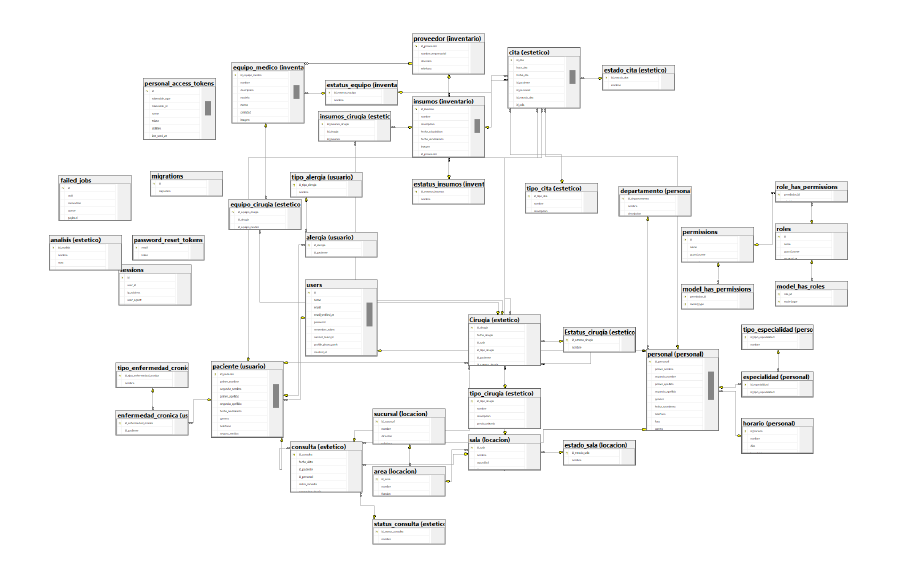
\includegraphics[width=0.7\textwidth]{img/data_base.png}
    \caption{Beautysys Database}
\end{figure}

Appointment Generation and Management:
The system will enable the efficient scheduling and tracking of appointments, offering flexibility for both patients and practitioners. Through intuitive interfaces and automated reminders, it aims to minimize scheduling conflicts and maximize clinic utilization.
\newline
Consultation Records and Documentation:
Detailed records of patient consultations will be meticulously stored, providing a comprehensive overview of each individual's medical history, preferences, and treatment plans. This ensures continuity of care and facilitates informed decision-making for both patients and medical professionals.
\newline
Surgical Procedures Management:
From pre-operative assessments to post-operative follow-ups, the system will streamline the entire surgical process, maintaining meticulous records of procedures performed, surgical outcomes, and patient recovery progress. This comprehensive approach enhances patient safety and enables continuous improvement in clinical practices.
\newline
Inventory Control and Management:
In addition to clinical data, the system will incorporate robust inventory management functionality, allowing for the seamless tracking and replenishment of medical supplies, implants, and consumables. By maintaining accurate inventory records, the clinic can optimize resource utilization, minimize waste, and ensure timely procurement of essential items.
\newline
Integration and Data Security:
To ensure seamless operation and data integrity, the system will feature robust integration capabilities, allowing for seamless communication with existing clinic infrastructure and external stakeholders. Moreover, stringent security measures will be implemented to safeguard patient confidentiality and protect against unauthorized access or data breaches.

\section{Operating Environment}
The website will be operate in any Operating Environment - Mac, Windows, Linux etc. 

\section{Design}

\begin{figure}[H]
    \centering
    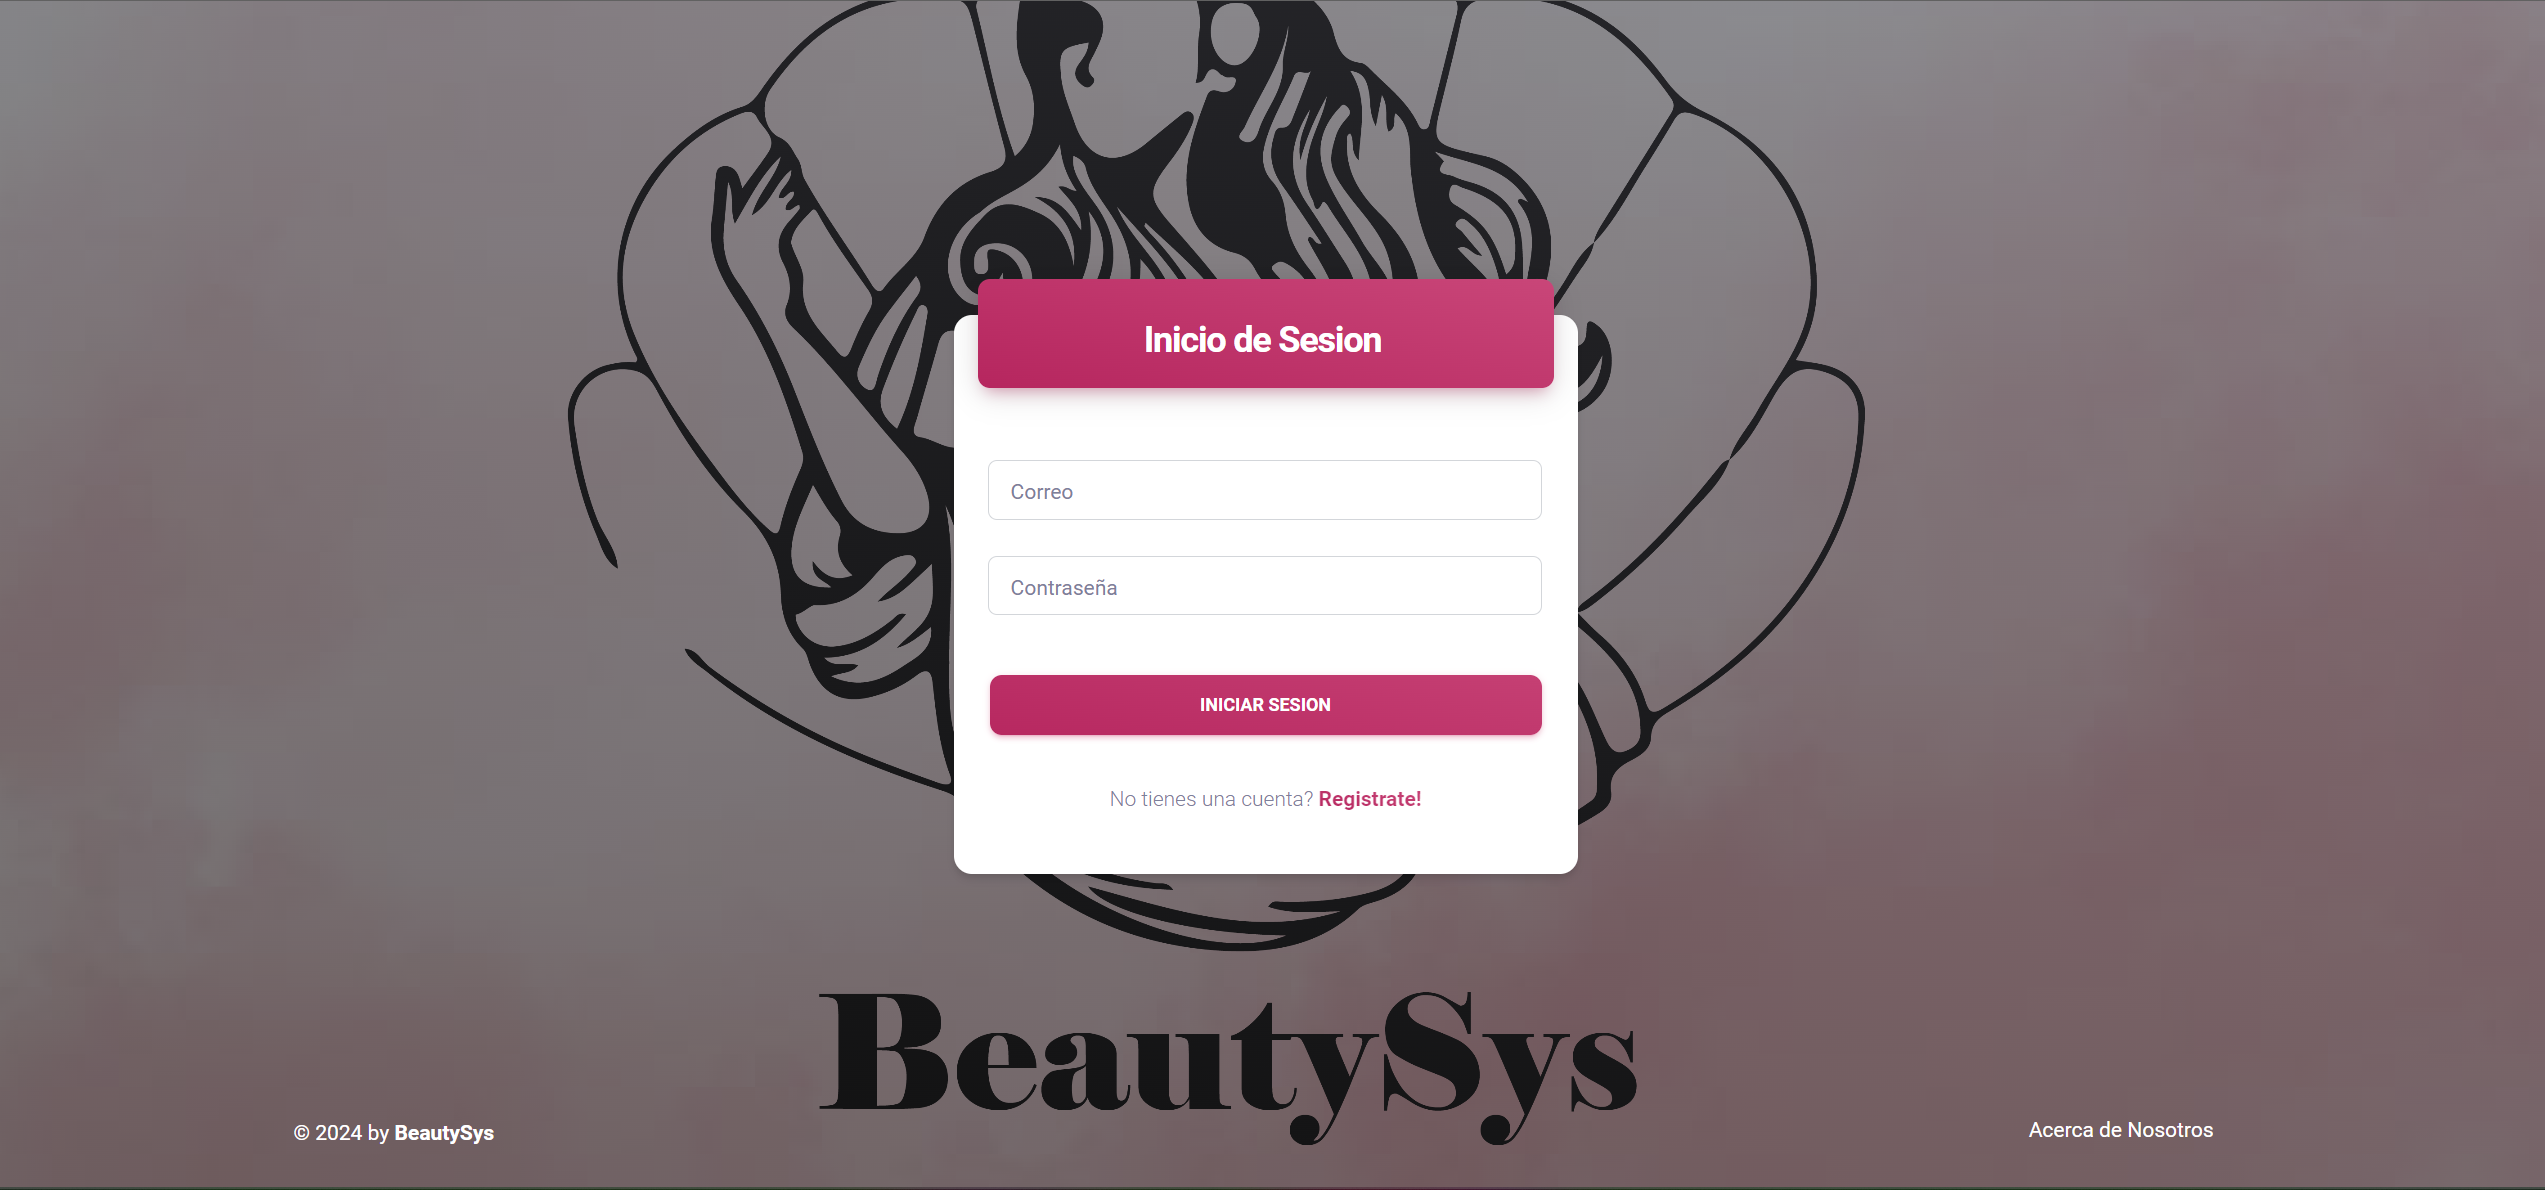
\includegraphics[width=0.7\textwidth]{img/Login_Page.png}
    \caption{Beautysys Login Page}
\end{figure}

\begin{figure}[H]
    \centering
    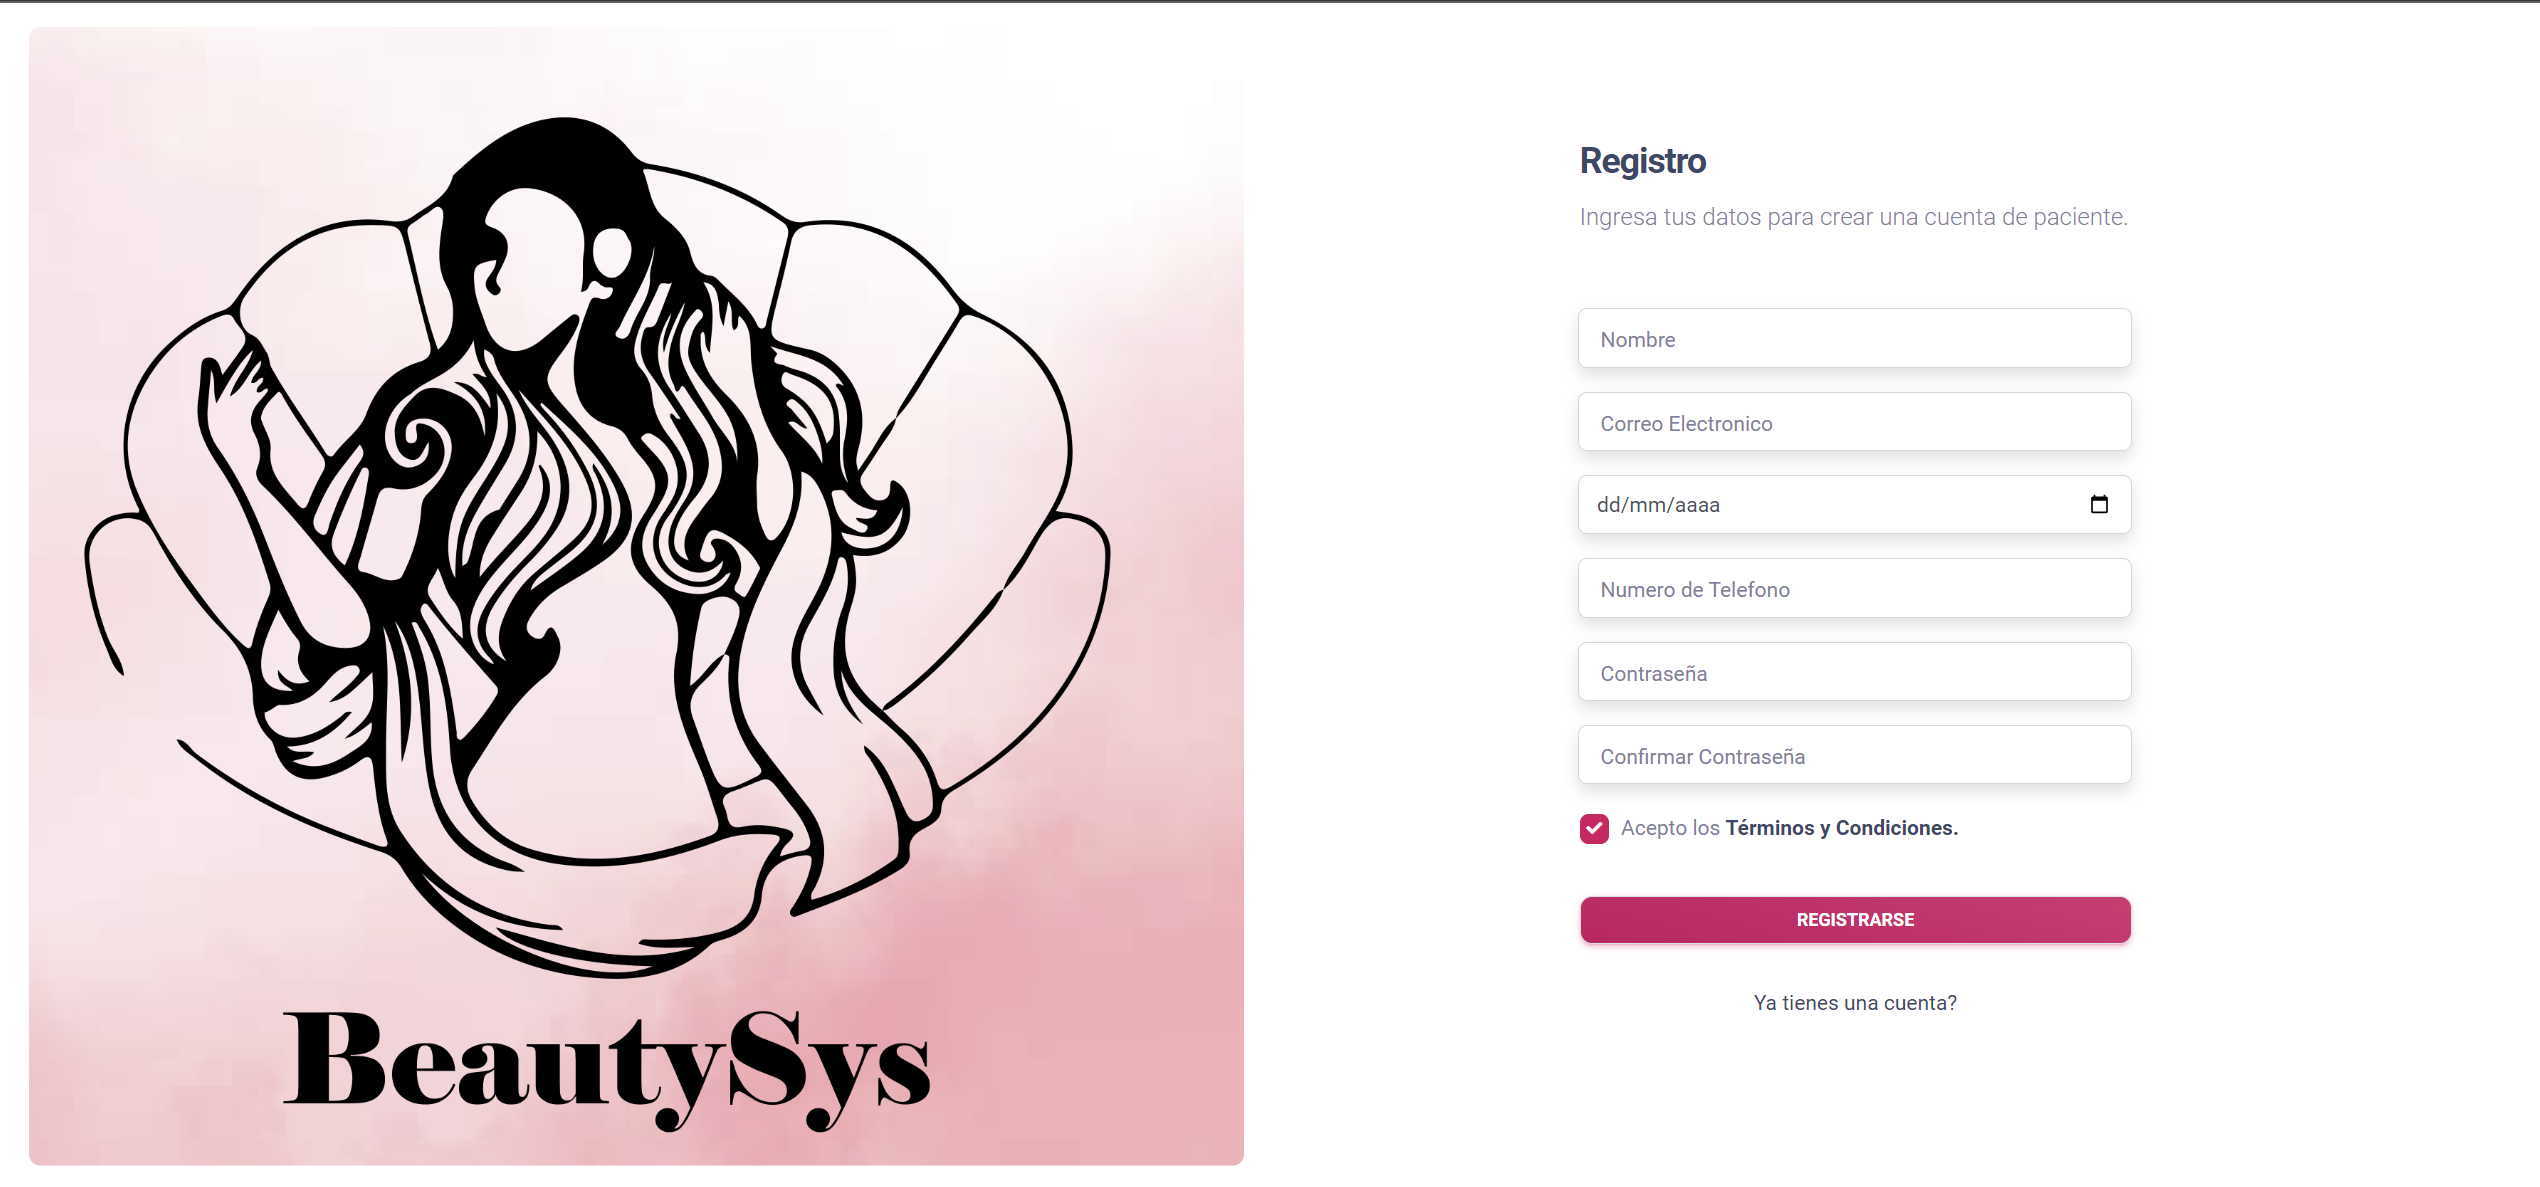
\includegraphics[width=0.7\textwidth]{img/Register_page.png}
    \caption{Beautysys Register Page}
\end{figure}

\begin{figure}[H]
    \centering
    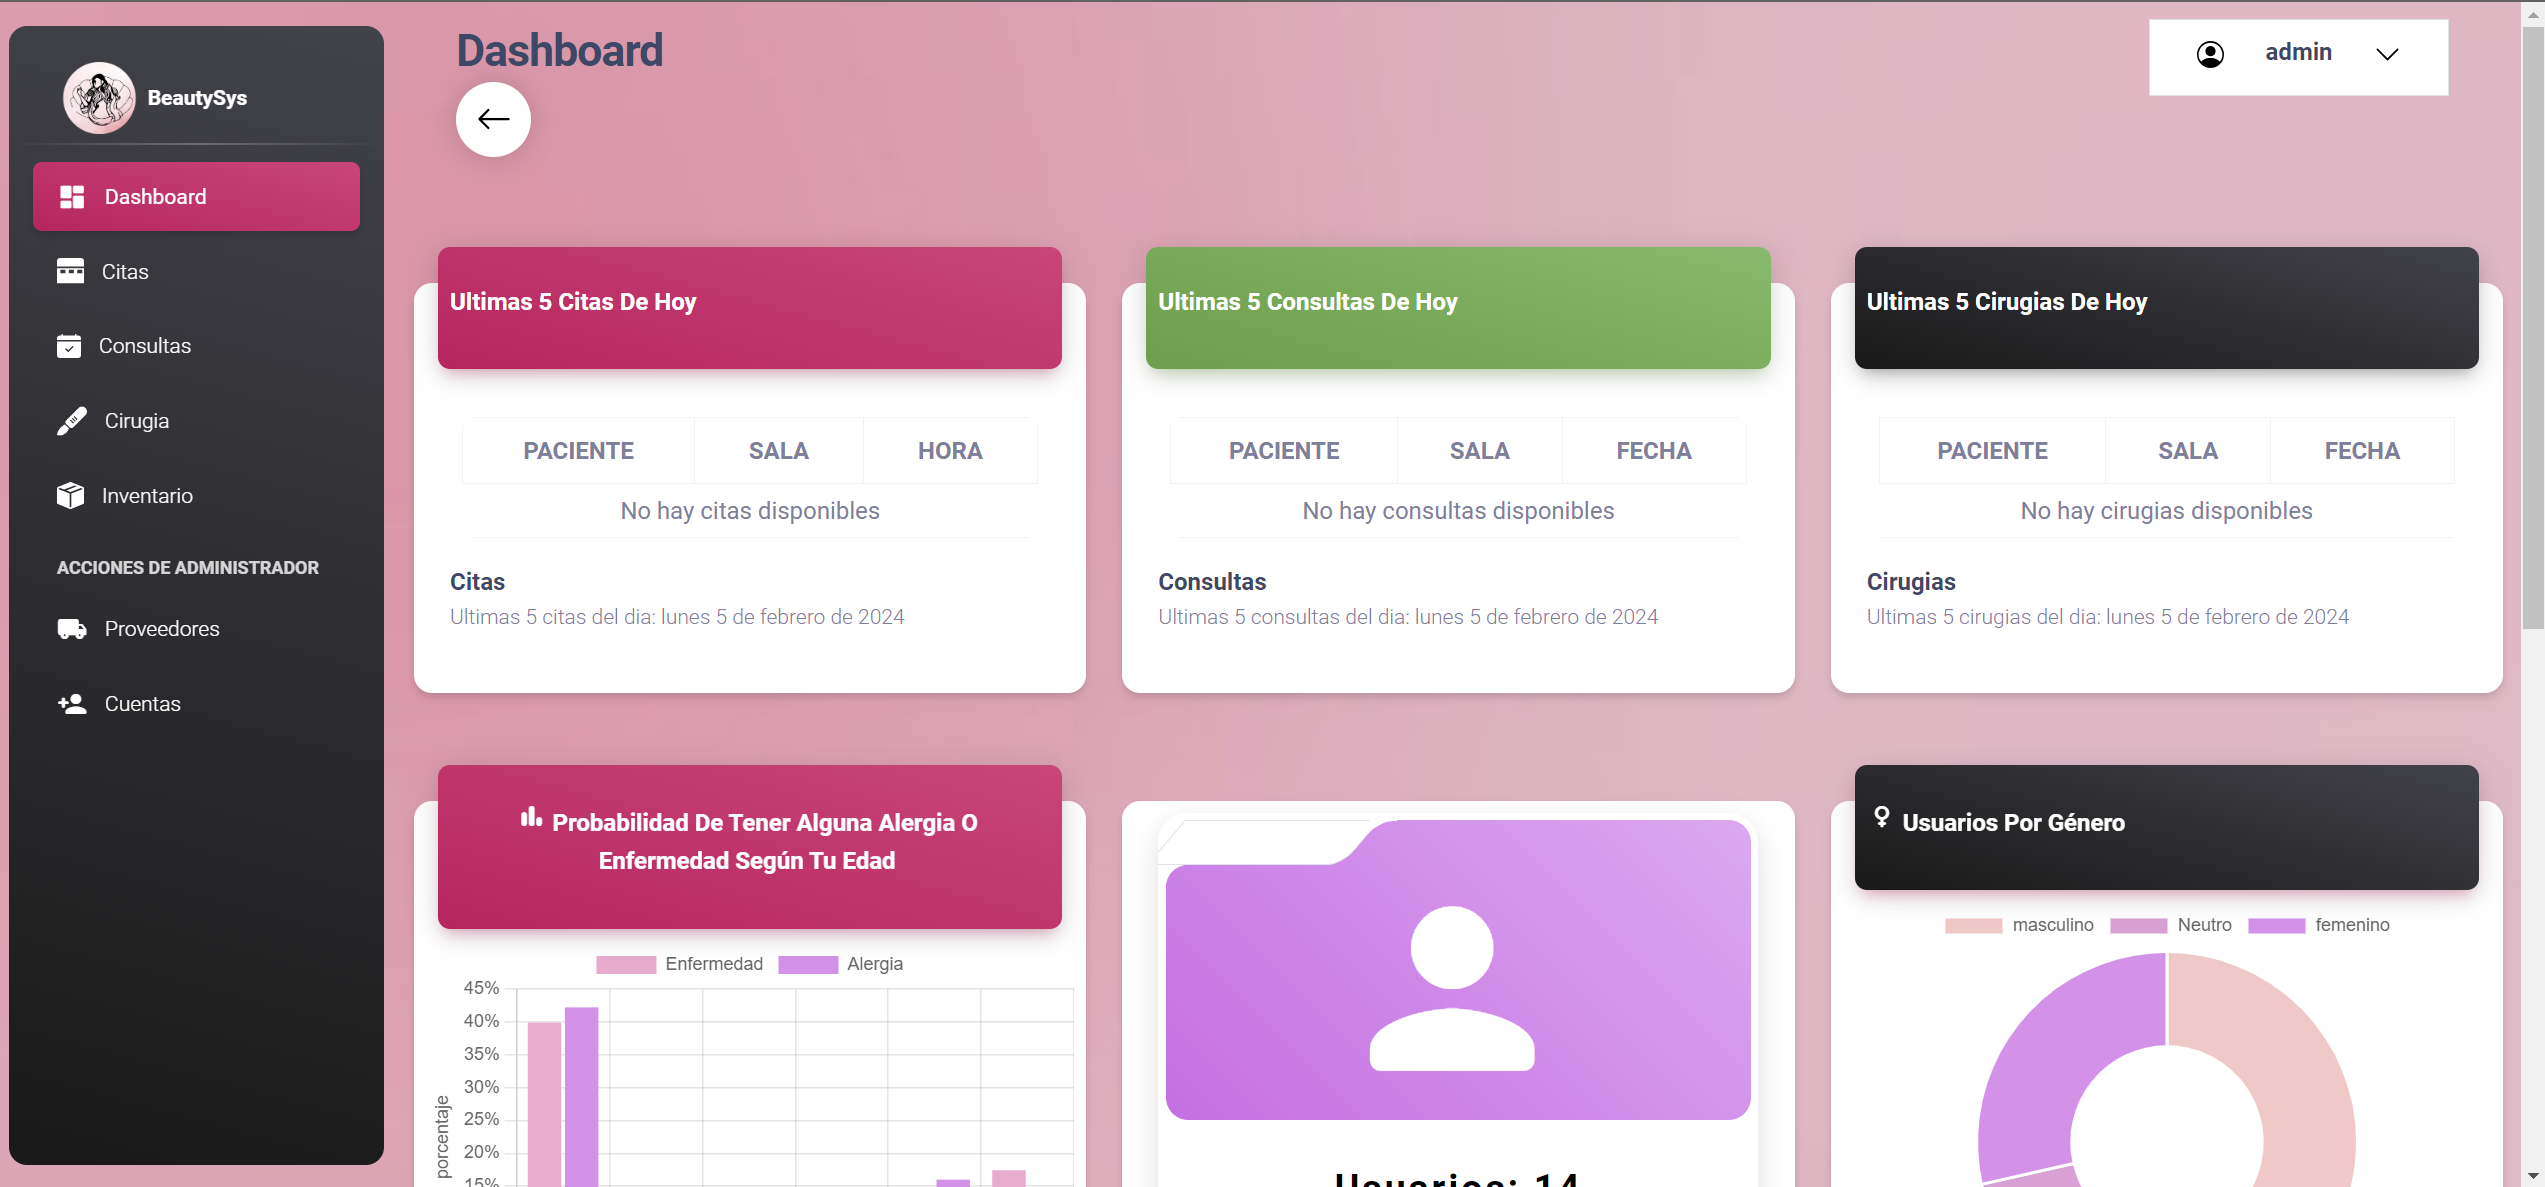
\includegraphics[width=0.7\textwidth]{img/home_page.png}
    \caption{Beautysys Dashboard} 
\end{figure}

\begin{figure}[H]
    \centering
    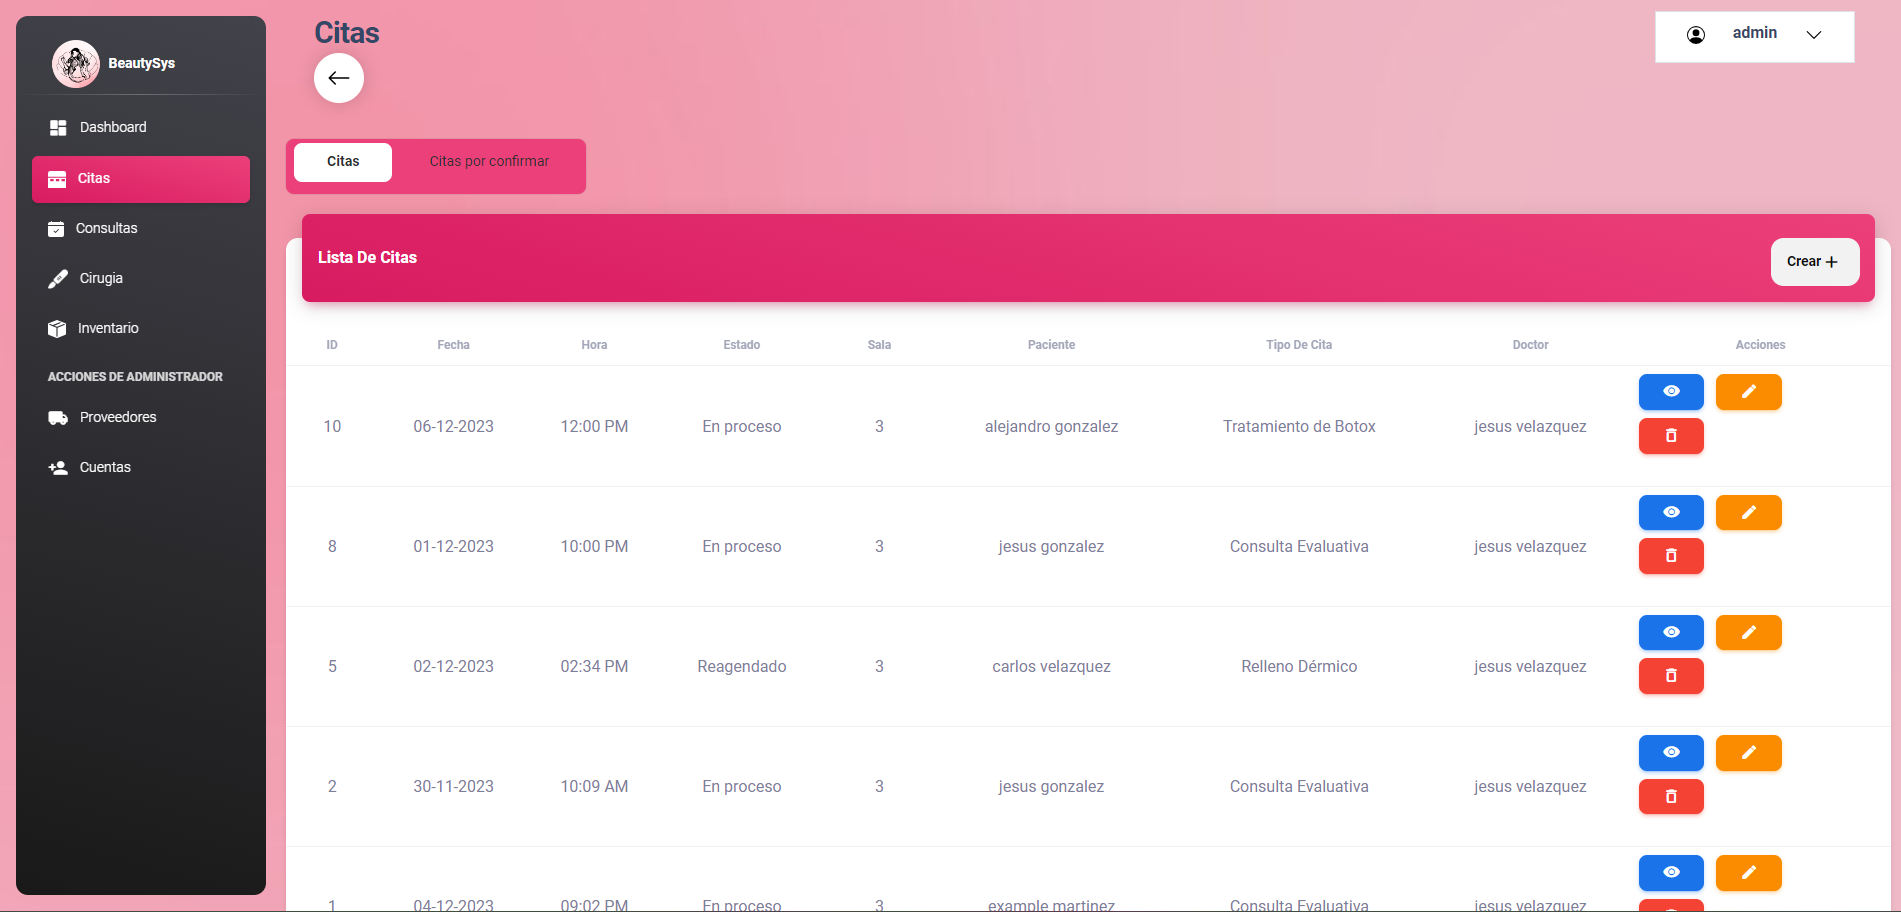
\includegraphics[width=0.7\textwidth]{img/citas_home.png}
    \caption{Beautysys Citas Page}
\end{figure}

\begin{figure}[H]
    \centering
    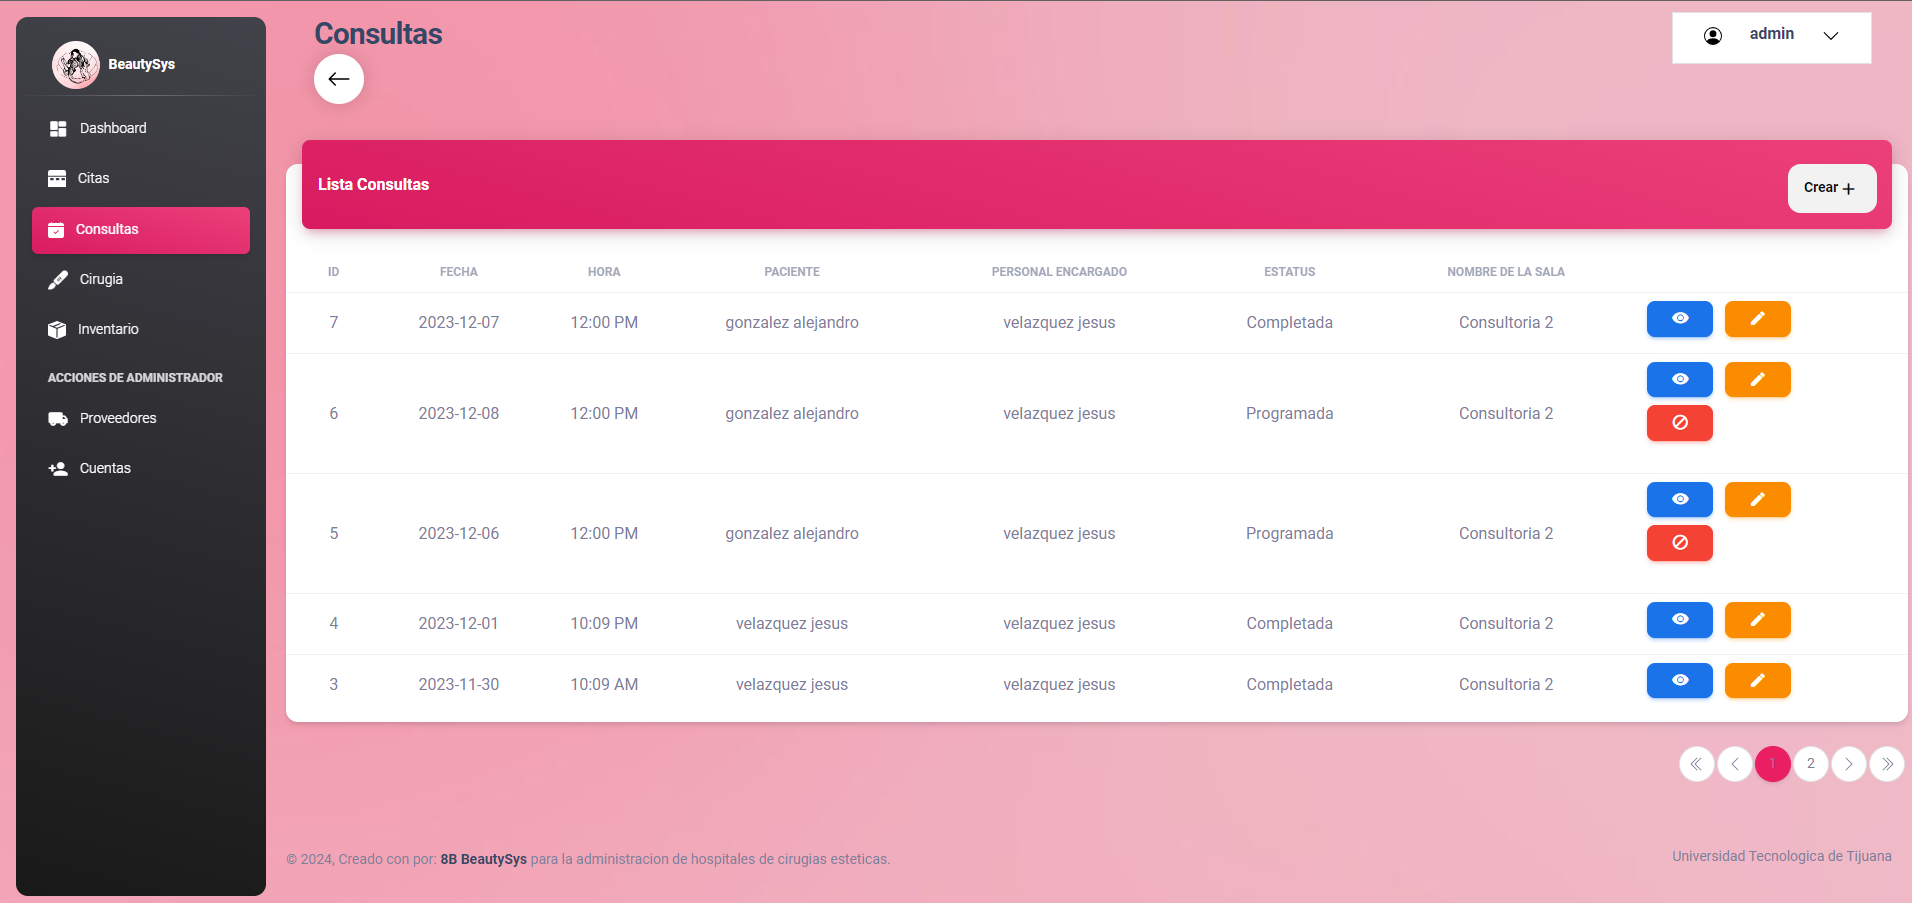
\includegraphics[width=0.7\textwidth]{img/Consultas_home.png}
    \caption{Beautysys Consultas Page}
\end{figure}


\begin{figure}[H]
    \centering
    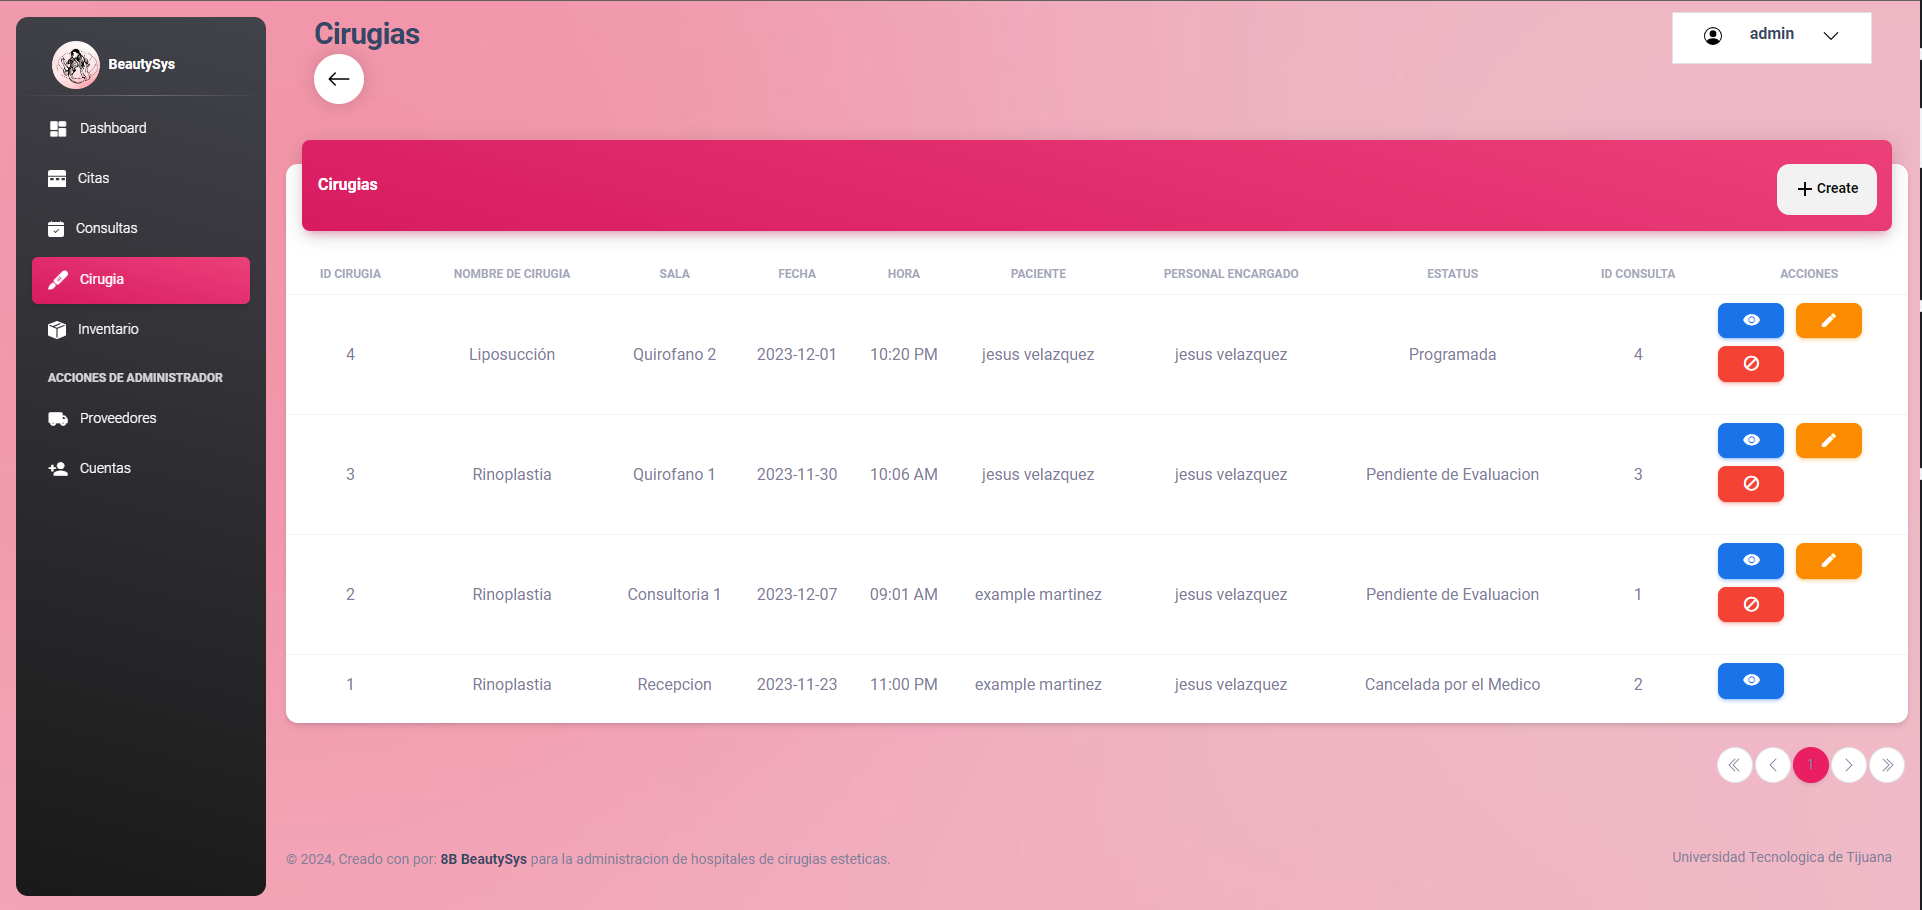
\includegraphics[width=0.7\textwidth]{img/Cirugias_home.png}
    \caption{Beautysys Cirugias Page}
\end{figure}

\begin{figure}[H]
    \centering
    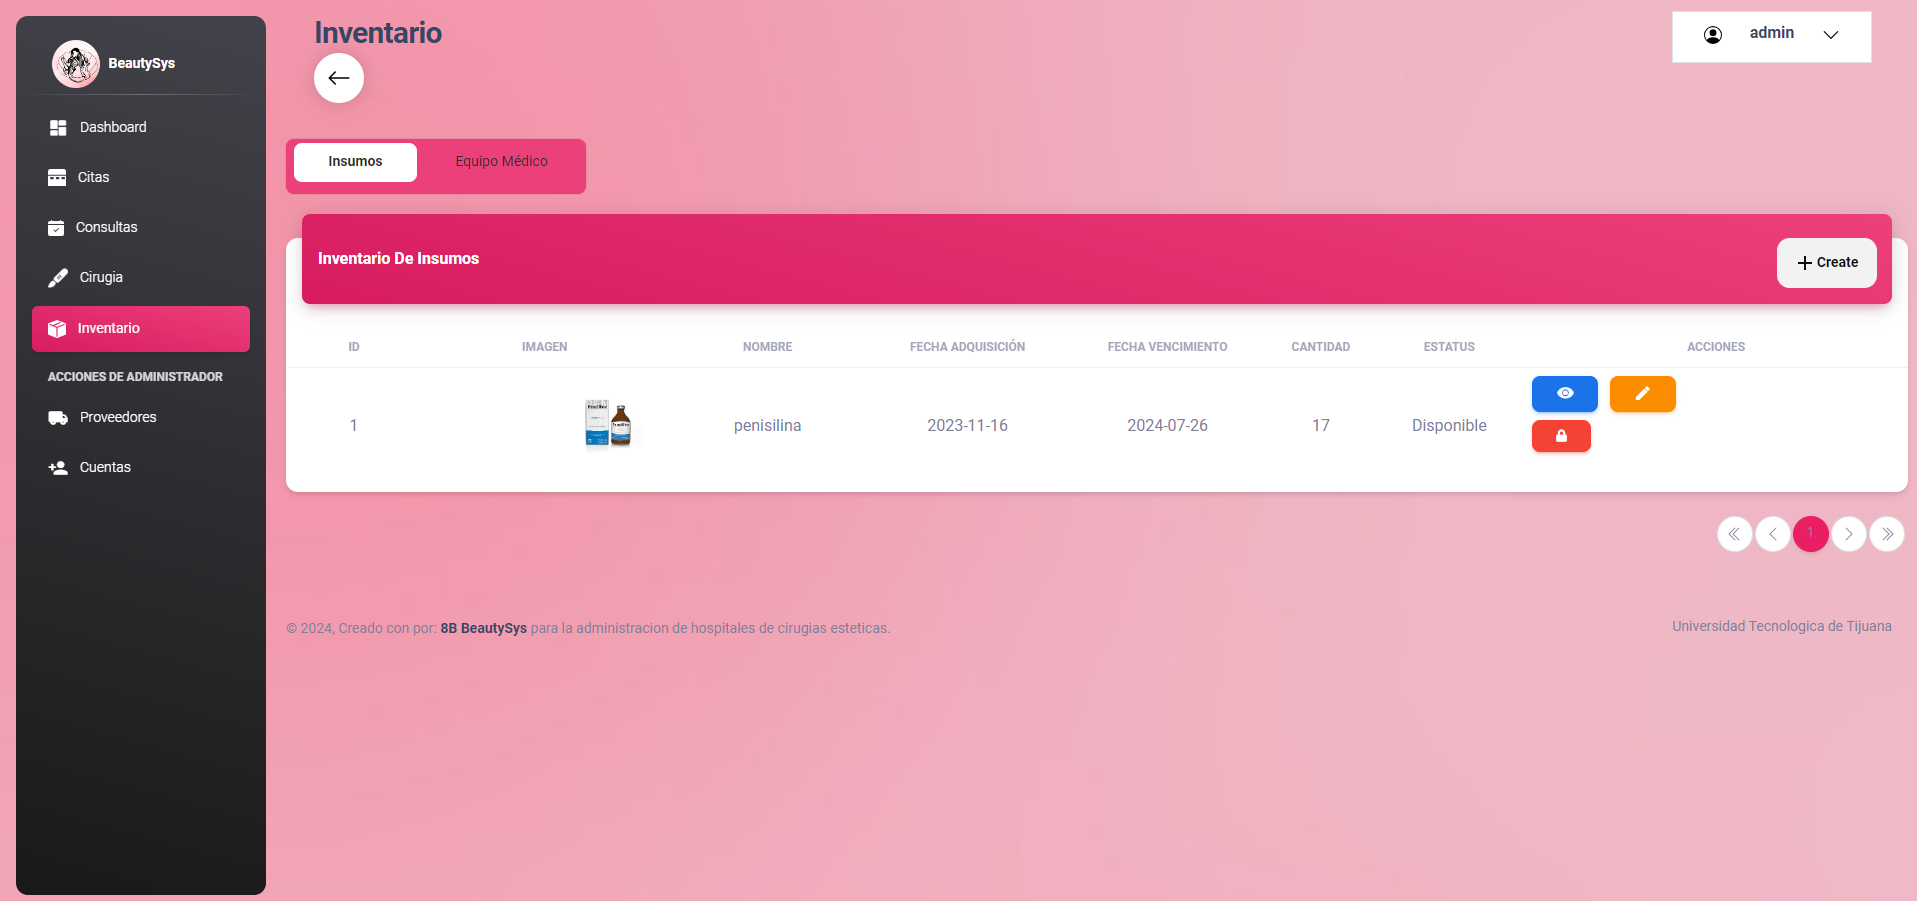
\includegraphics[width=0.7\textwidth]{img/Inventario_home.png}
    \caption{Beautysys Inventario Page}
\end{figure}

\begin{figure}[H]
    \centering
    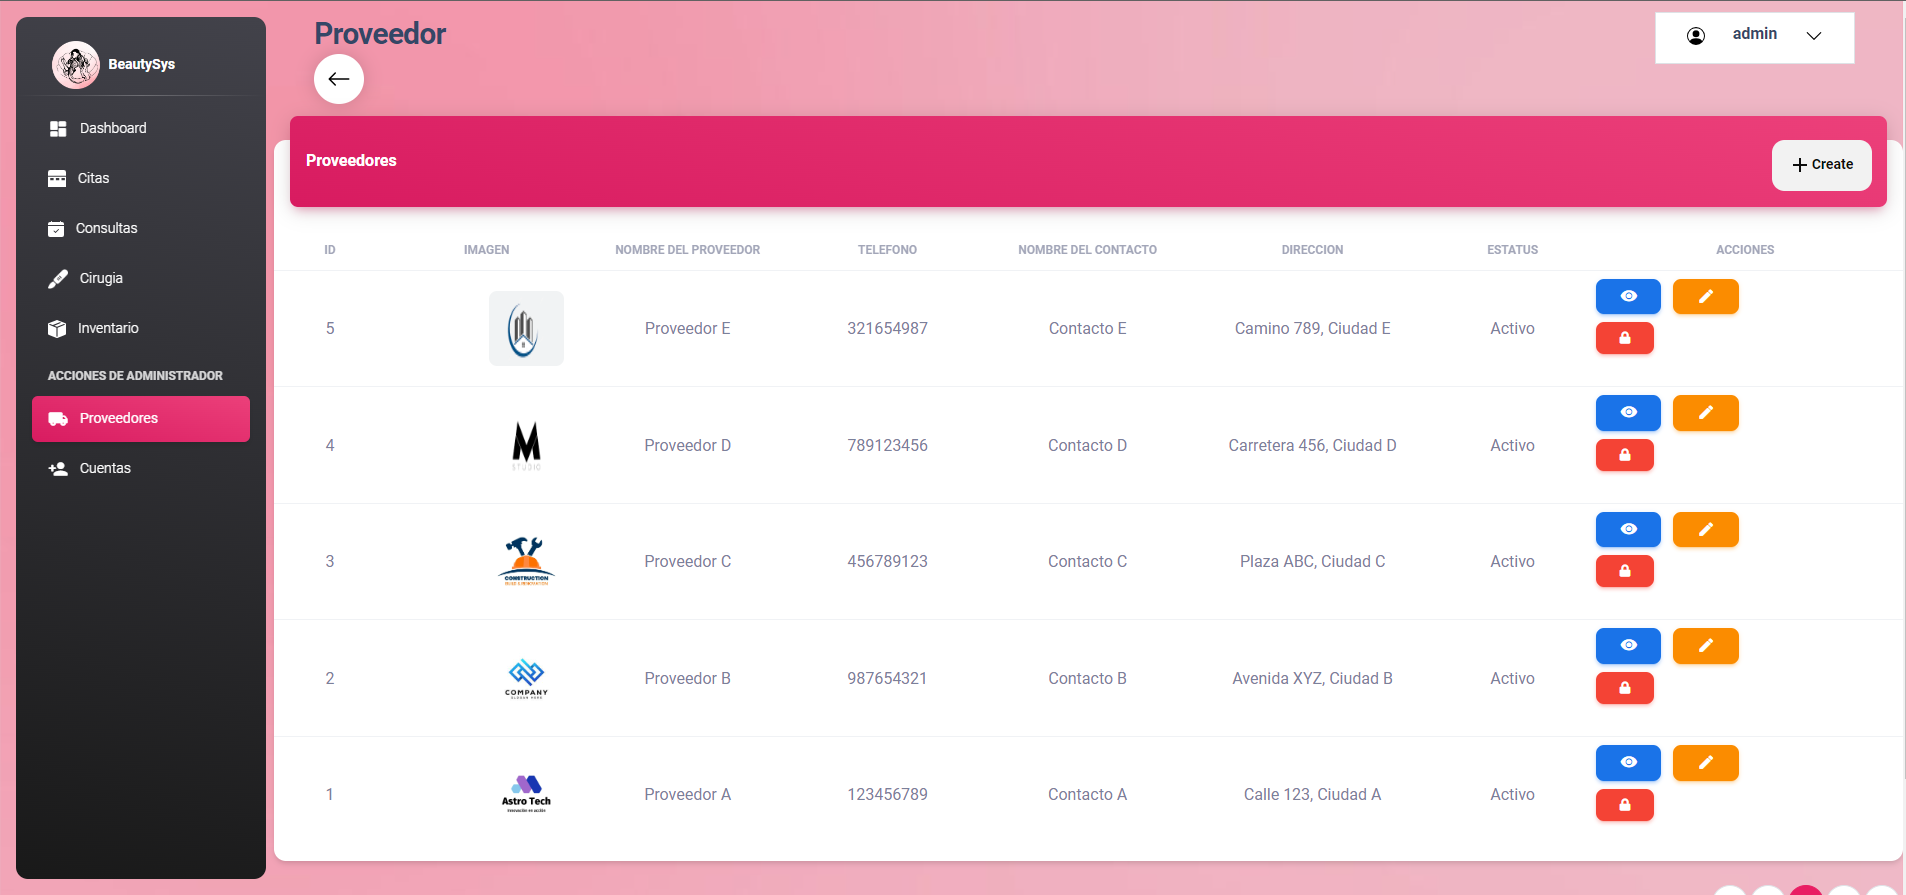
\includegraphics[width=0.7\textwidth]{img/Proveedor_home.png}
    \caption{Beautysys Proveedor Page}
\end{figure}

\begin{figure}[H]
    \centering
    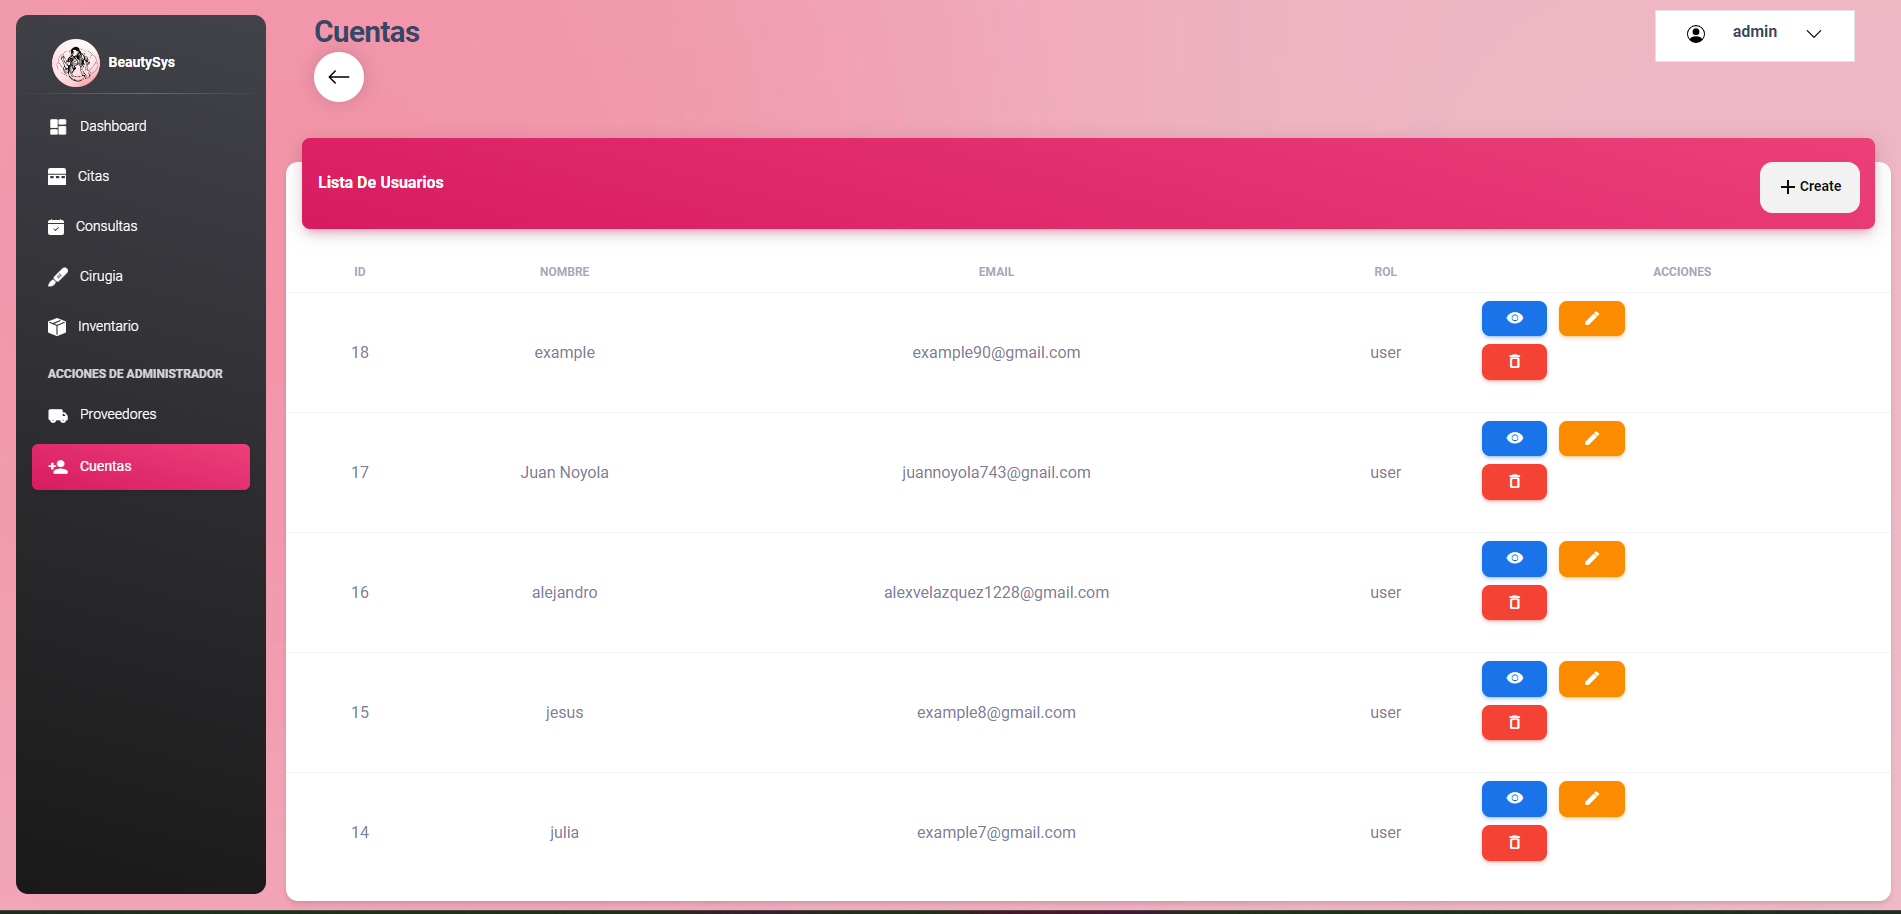
\includegraphics[width=0.7\textwidth]{img/Cuentas_home.png}
    \caption{Beautysys Cuentas Page}
\end{figure}

\section{UML}

\begin{figure}[H]
    \centering
    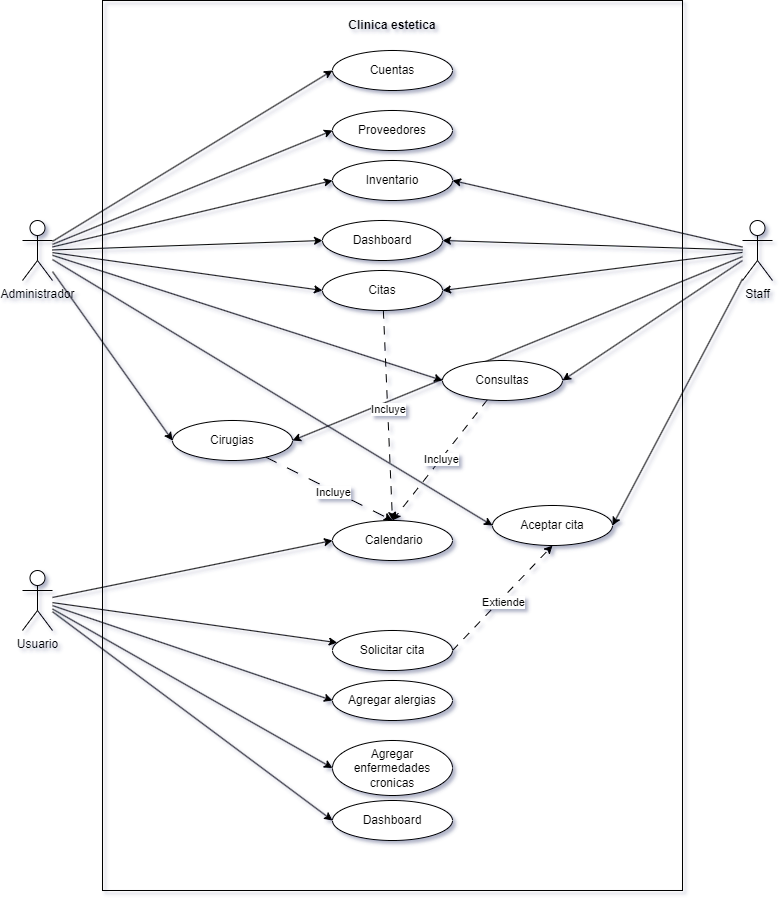
\includegraphics[width=0.9\textwidth]{img/UML.png}
    \caption{Beautysys UML Diagram}
\end{figure}

\chapter{System Features}
"BEAUTYSYS WEBSITE" is conceived with the primary goal of enhancing efficiency in the process of recording, accessing, and modifying data, while concurrently bolstering data security measures and elevating the standard of customer care. By streamlining these essential functions, the system aims to provide a seamless experience for both clinic staff and clients, fostering trust and satisfaction.

\section{Description and Priority}
"BEAUTYSYS WEBSITE" has features that are main and also some are sub. But all the feature is necessary for this software.

\begin{enumerate}
\item Appointment Generation and Management: The system will enable the efficient scheduling and tracking of appointments, offering flexibility for both patients and practitioners. Through intuitive interfaces and automated reminders, it aims to minimize scheduling conflicts and maximize clinic utilization.

\item Consultation Records and Documentation: Detailed records of patient consultations will be meticulously stored, providing a comprehensive overview of each individual's medical history, preferences, and treatment plans. This ensures continuity of care and facilitates informed decision-making for both patients and medical professionals.

\item Surgical Procedures Management: From pre-operative assessments to post-operative follow-ups, the system will streamline the entire surgical process, maintaining meticulous records of procedures performed, surgical outcomes, and patient recovery progress. This comprehensive approach enhances patient safety and enables continuous improvement in clinical practices.

\item Inventory Control and Management: In addition to clinical data, the system will incorporate robust inventory management functionality, allowing for the seamless tracking and replenishment of medical supplies, implants, and consumables. By maintaining accurate inventory records, the clinic can optimize resource utilization, minimize waste, and ensure timely procurement of essential items.

\item Integration and Data Security: To ensure seamless operation and data integrity, the system will feature robust integration capabilities, allowing for seamless communication with existing clinic infrastructure and external stakeholders. Moreover, stringent security measures will be implemented to safeguard patient confidentiality and protect against unauthorized access or data breaches.
\end{enumerate}

\section{Functional Requirements}
The "BEAUTYSYS WEBSITE" is being build on Laravel framework and SQL server
\newline
Back-End - Laravel.
\newline
Font-End - Laravel.
\newline
Database -  SQL server.


\chapter{Other Nonfunctional Requirements}

\section{Performance Requirements}
"BEAUTYSYS WEBSITE" will be used for a comprehensive system for the monitoring, management and administration of a cosmetic surgery clinic. So, for further interaction, Laravel and SQL Server are used.

\section{Security Requirements}
No one without registered users can inter to the website. One particular user of a section only can perform his/her particular actions. 

\section{Software Quality Attributes}
In the development phase also testing and conferences of users is been continued. So that the quality of the software is been maintained and all the requirements are been fulfilled.
\newline
Database, logical and also UI test is required. 

\section{Business Rules}
"BEAUTYSYS WEBSITE" is a comprehensive system for the monitoring, management and administration of a cosmetic surgery clinic.
\newline
Basically save working time and pressure. 


\chapter{Other Requirements}
"BEAUTYSYS WEBSITE" needs maintenance as it is a long process software. It will need re-factoring and further the requirements can be changed as the field is changing frequently. 

\end{document}